\documentclass[9pt,twocolumn,twoside,lineno]{gsajnl}
% Use the documentclass option 'lineno' to view line numbers

\usepackage{epstopdf}

\articletype{inv}
% article type
% {inv} Investigation
% {gs} Genomic Selection
% {goi} Genetics of Immunity
% {gos} Genetics of Sex
% {mp} Multiparental Populations

\runningtitle{GENETICS Journal Template on Overleaf} % For use in the footer
\runningauthor{FirstAuthorLastname \textit{et al.}}

\title{COMP9727 Recommender Systems Report}

\author[1]{Jinghan Wang  z5286124}

\begin{abstract}
The article focuses on implementing and evaluating a complex news recommendation system using the MIND (Microsoft News Dataset) dataset. The methods used include Factorization Machines (LibFM), Neural Collaborative filtering (NCF), matrix factorization (MF), graph neural networks (GNN), and advanced deep learning models. An attempt is made to utilize the models mentioned above to improve the accuracy and efficiency of the news recommendation system and to increase user engagement and satisfaction in digital news consumption.
\end{abstract}

\keywords{6643}

\dates{\rec{20 09, 2022} \acc{10 10, 2022}}

\begin{document}

\maketitle
\thispagestyle{firststyle}
%\slugnote
%\firstpagefootnote
\vspace{-13pt}% Only used for adjusting extra space in the left column of the first page

\section{Introduction}
\subsection{Project Background}
The way people consume news has changed dramatically, moving from conventional print media to digital channels. In the past, print magazines and television shows were the main ways that conventional media sources controlled the flow of news. But the modern digital age, marked by the expansion of mobile devices and the abundance of online news sources, has given individuals the ability to customise how they consume news.

For news media companies, this shift poses serious issues, especially when it comes to user engagement measures. Because click-through rates are frequently related to advertising income, they have become a crucial aspect. As a result, news organisations have to balance the need to provide interesting, pertinent material with user interaction optimisation.

Personalized news recommendation systems have become a viable answer to these problems. These systems utilize algorithms to select and recommend content according to the reading habits and personal preferences of each user. When compared to other recommendation contexts like entertainment media, the news domain poses distinct obstacles for the deployment of such systems.

News recommendation systems are characterised by many fundamental differences:

\begin{enumerate}
\item Content Volatility: News stories have a much shorter lifespan than other types of media. Recommendation algorithms need to be updated often due to the fast turnover of material.
\item Temporal Relevance: News material frequently exhibits significant temporal patterns, with some subjects (like election coverage) being more popular during particular eras and then rapidly going out of style afterward.
\item Cold Start Issue: Systems must quickly integrate and promote new items due to the transitory nature of news material, which exacerbates the cold start issue.
\item Implicit input mechanisms: Although news websites usually rely on implicit user input, mostly in the form of click behavior, some digital platforms make use of explicit rating systems.
\end{enumerate}

In 2000, Microsoft launched the Microsoft News Dataset \cite{webteam@eso.org} to support studies in this area. The purpose of this sizable dataset is to aid in the research of custom news recommendation algorithms. Microsoft used the dataset to host a research competition after it was released, and this has since sparked a great deal of scholarly interest. 133 scholarly articles have been published to date, covering a range of dataset features and different approaches to news recommendation.

The goal of the current research in this area is to improve the effectiveness of personalised content distribution in the digital news ecosystem while addressing the particular difficulties faced by news recommendation systems.

\subsection{Project Domain and Intended Users}
Online news is the realm of the recommendation system. If we define the term more precisely, we refer to online news sources such as Microsoft News, Google News, Yahoo News, and others. The target audience consists of people who regularly read news and would like customized material to be sent to them depending on their reading preferences.
 
and inclinations. These consumers frequently use their laptops or mobile devices to read the news. By suggesting news stories that match their interests, the system seeks to improve the user experience and increase user engagement, contentment, and loyalty.

\subsection{Number of Items Presented, User Interface and User Feedback}
The front page, which is the first page that customers see when they open the news app or website on their laptop, is the main emphasis of the user interface of the recommender system. The home page's design strives to deliver news in an aesthetically pleasing and easily navigable way. The website banner will appear at the top of the page. Some of the best news articles of the day will be featured in it. The news in the banner usually has an eye-catching headline and eye-catching pictures. We often see news divided into many sections below the banner. The news title and an abstraction of some key phrases for each category will be displayed.

Quite a lot of news will be posted on this type of home page. According to the data set analysis, each "impression" consists of an average of 37.4 news items. One time a user is shown a selection of news stories, it is referred to as an "impression." When the reader views the home page or reloads it, this will happen. Every impression will include the news ID of the item of news that is displayed, together with the user's click-through rate.

Whether or not the user clicks on the news is the primary kind of feedback. There is no clear scoring system for news stories. Usually, the common approach is implicitly deduced from the click behaviors.

\subsection{Business Model and Revenue Generation}
A system like this would include subscription, advertising, and data insights and analytics as its main income streams.

Subscription services are offered by websites such as The Wall Street Journal in order to access premium news and analysis. A membership offers users access to unique content and an ad-free experience. In contrast, public audiences are the focus of platforms such as Microsoft News and Google News. To make money, they include ads in their news articles. These advertisements aren't made at random. Personalized advertisements tend to have higher click-through rates. Another important source of income will come from providing publishers and marketers with data insights and analytics services. Through the analysis of content performance and user interaction,
 
The platform has the ability to provide insightful data that helps stakeholders improve their strategy.

Similarly to what happens on Microsoft News, the project's website will offer free news. In addition, advertising and data insights and analytics will bring in money.

\section{Dataset}
\subsection{Background and Data Structure}
The behavior records of a million people who clicked on news stories at least five times in the six weeks between October 12 and November 22, 2019, are included in the MIND data set. Only the hash ID of each user, who has been disconnected from the production system, is included in the dataset.
\begin{itemize}[noitemsep]
  \item The data of the sixth week are used for the test.
  \item The data from the fifth week are used for training.
  \item The data from the last day of the fifth week are used for validation.
\end{itemize}
The data set has already been split. In each folder, it contains the following 4 files,
\begin{itemize}[noitemsep]
  \item \texttt{behaviors.tsv} with the click histories and impression logs of users.
  \item \texttt{news.tsv} containing news article information. Additionally, the news URL is given so that we may scrape the news content and incorporate it into the modelling. Nevertheless, some URLs have already expired because the news articles are at least 4 years old, which implies the experiments could no longer be able to operate on the news content. This shouldn't be too concerning because when a visitor accesses the home page, they mostly read the headline, abstract, and keywords before determining whether or not to click to explore additional content.
  \item \texttt{entity-embedding.vec} and \texttt{relation\_embedding.vec}. The entities and relations that were learnt from the WikiData knowledge graph are encoded in these two files in a 100-dimensional format. Said another way, the embeddings on a big knowledge graph reflect the vector of that news. These two attributes have the potential to aid in the investigation of knowledge-aware news recommendation.
\end{itemize}

\subsection{Preliminary Analysis}
Table \ref{tab:1} provides an overview of the total number of records in the data collection.

A total of 161,013 news items and 1 million user records are present. According to the preceding paragraph, the dataset includes people who clicked on at least five news items throughout the six-week period. Duplicate usage IDs are therefore common in the data set.

\subsubsection{Behaviors\newline}
A snapshot of the \texttt{behaviors.tsv} file is shown in Table \ref{tab:2}. Every ID in the history column corresponds to a news item. Additionally, each ID in the impressions column denotes a news item and a click status; a click status of 1 indicates that the news item has been clicked, while a click status of 0 indicates that it has not. After the user is given the "history," each row indicates the click state.


The dataset that is being examined has 2,232,748 records in total, more than 2.2 million entries, and 711,222 unique users have been identified. This disparity suggests that many users have several related records. A workable solution for the 46,065 entries with blank history fields would be to substitute the most recent historical information from the relevant user for these null values. The dataset documentation states that during a six-week period from October 12 to November 22, 2019, 1 million people who had at least five news clicks were chosen as part of the sample technique. The news click history was constructed using click behaviors observed throughout the first four weeks to model user behavior. The samples taken on the last day of the fifth week make up the validation set. The training set includes data from November 9, 2019, from 00:00 hours, to November 14, 2019, at 23:59 hours, according to statistical analysis. Data from November 15, 2019 make up the validation set, while data from November 16, 2019, from 00:00 hours to November 22, 2019, at 23:59 hours, make up the test set. As a result, the training set includes data for six days. Users have historically been exposed to an average of 33.67 news items, whereas the impression set has an average of 37.40 news items.

\subsubsection{New\newline}
Table \ref{tab:3} displays a snapshot of the \texttt{news.tsv} file. Every news item has a title, an abstract, a URL, a major category, and a subcategory. After that, there are a title entity and an abstract entity composed of extra keys. The \texttt{entity\_embedding.vec} and \texttt{relation\_embedding.vec} files are used to map these entities to embed vectors.

One News\_ID (a unique identifier), Category, Subcategory, Title, Abstract, URL, Title Entities, and Abstract Entities are among the eight unique fields present in each of the 101,527 news items that make up the collection. In particular, the 2019 URLs are now mostly unavailable, making content-based model training impossible. 

\begin{figure}
    \centering
    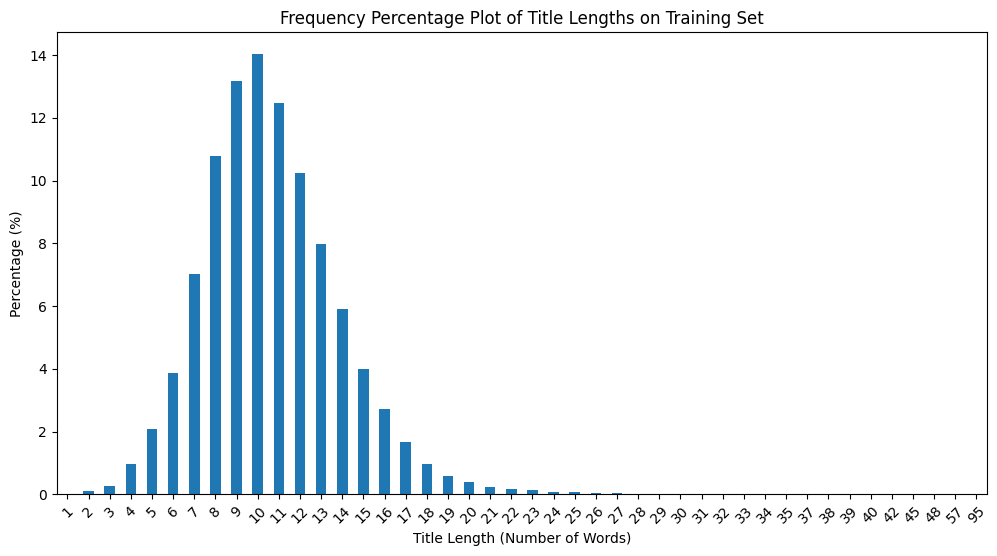
\includegraphics[width=\linewidth]{material/1.png}
    \caption{Frequency Percentage Plot of Title Lengths}
    \label{fig:1}
\end{figure}

In addition, it emphasizes the length of the title, which is important to retain users. shows the distribution of news title lengths on the training site. Figure \ref{fig:1} indicates that most news titles are concise, with a peak of about 9 - 10 words. This indicates that users are often exposed to brief and to-the-point headlines. That means a striking topic will help increase the clicking rate. 

\begin{figure}
    \centering
    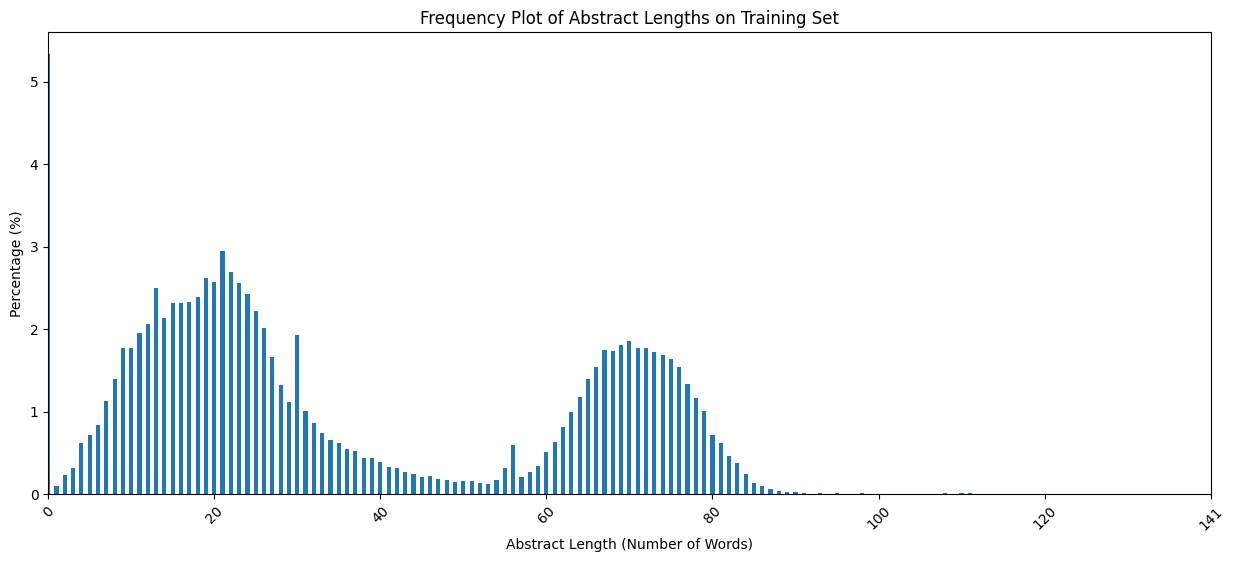
\includegraphics[width=\linewidth]{material/2.png}
    \caption{Frequency Plot of Abstract Lengths}
    \label{fig:2}
\end{figure}

The distribution of abstract lengths for the new articles in the training set is shown in Figure \ref{fig:2}. In the graph, there are two peaks. Twenty words or so make up the initial leak. The second peak has a word count of about 70. The bimodal distribution indicates that there may be a significant variation in the length of news abstracts due to the various categories or kinds of article. The model has to handle different quantities of text data because there are short and extensive abstracts.

\subsubsection{Survival Time\newline}
The "survival time" is a fascinating term in the study of news data. The time span between the first and last appearances of a news item is the definition of this statistic. Because the results obtained from the dataset are based only on impression timestamps rather than real publishing or retraction periods, it should be emphasized that they may include some degree of error. Still, this method yields a decent approximation of the news lifetime in the system.

\begin{figure}
    \centering
    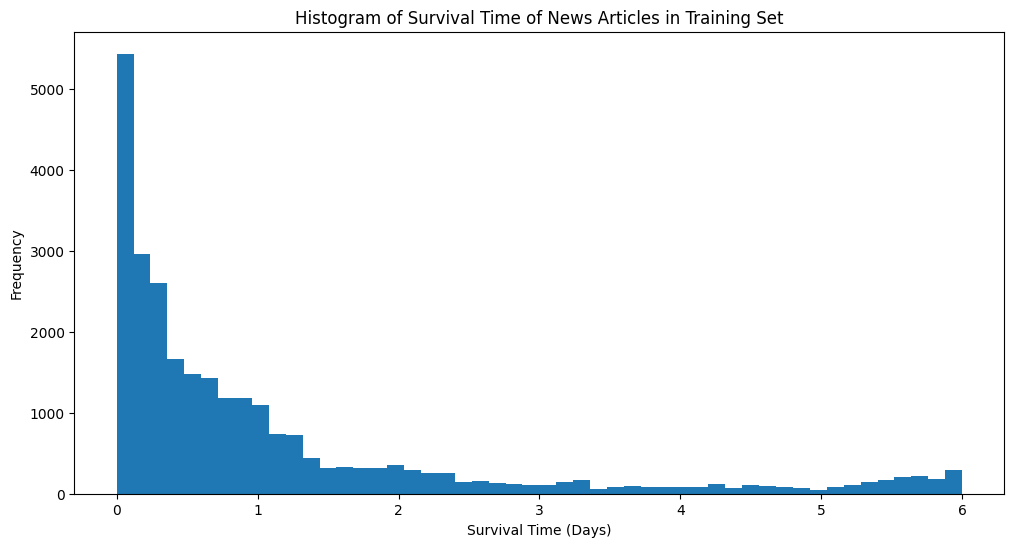
\includegraphics[width=\linewidth]{material/3.png}
    \caption{Histogram of Survival Time of News Articles}
    \label{fig:3}
\end{figure}

The survival time distribution of the training dataset is shown in Figure \ref{fig:3}. The plot shows that the vast majority of news stories—roughly 70\%—only receive clicks on the day they are published, with the interaction dropping dramatically after the first 24 hours. This fast decay pattern is consistent with a Poisson distribution, which is a frequent occurrence in temporal data analysis.

The trend that has been noticed highlights how dynamic news consumption habits are, as well as how difficult it is for news recommendation systems to get off the ground quickly. This result highlights how important it is for recommendation engines to successfully promote news information within a constrained timeframe, before the articles' value and relevance dwindle.

The information indicates that the best way to maximize the interaction of the article is to use timely and effective content marketing techniques. This discovery also emphasizes how critical it is to create recommendation algorithms that can quickly adjust to freshly released information to solve the cold-start issue in the context of news recommendation systems.

\subsection{Challenge}
This study uses the MINDsmall dataset due to the large size of the original dataset and limited computer resources. However, the tiny validation set could not be downloaded; only the training version of the data set was available. In order to overcome this restriction, a data extraction technique was developed that pulls pertinent information from the original data set using the user\_id from the training data set.

Consistency was preserved during the data splitting procedure by keeping the same 50,000 users in the test and validation sets. The following data distribution was obtained using this method:

\begin{itemize}[noitemsep]
\item For validation: 22,880 instances were retained out of 255,990, representing 8.9% of the original validation set.
\item For testing: 140,593 instances were preserved out of 702,005, constituting 20% of the original test set.
\end{itemize}

These percentages imply a representative sample for evaluation purposes, since they show that the 50,000 users chosen had a substantial impact on the test set.

The filtered dataframes were stored in specified folders after the data extraction and splitting process. After manually moving more pertinent files to these directories, three separate datasets \texttt{MINDsmall\_train}, \texttt{MINDsmall\_dev}, and \texttt{MINDsmall\_test} were produced.

This method of data preparation guarantees a more controllable dataset while preserving a representative and varied sample for the news recommendation model development process' training, validation, and testing stages.

\section{Methods}
\subsection{Method 1: LightFM Hybrid Recommender System}
Combining the benefits of content-based and collaborative filtering, the LightFM model is an inventive approach to news recommendation systems.  Due to its hybrid design, the model can take advantage of content characteristics as well as user-item interaction data, offering a more complete recommendation framework.

\subsubsection{Model Type\newline}
A hybrid recommender system is what LightFM is categorised as.  It combines content-based filtering, which takes into account the characteristics of both things and users, with collaborative filtering, which makes use of patterns in user-item interactions.  This combination enables the model to get around the drawbacks of each technique when applied separately, such as the cold-start issue that frequently arises in solely collaborative systems.

\subsubsection{Data Input}
\begin{enumerate}
\item \textbf{Interaction Matrix}: The Interaction Matrix records past user interactions with news stories, usually in the form of clicks or views.
\item \textbf{Feature Matrices}: These matrices include extra information about both people and things (news articles).  This might include things like keywords, publishing sources, and topic categories for news stories.  User characteristics may include preferences that are explicitly mentioned or demographic information.
\item \textbf{User IDs}: Special numbers that only each user has in the system.
\item \textbf{News IDs}: Unique numbers assigned to every news item.
\item \textbf{TF-IDF vectors}: Comprising two parts, these vectors depict the substance of news articles:
    \begin{enumerate}
    \item Historical News Vector: This represents how the user has interacted with news items in the past.
    \item Current News Vector: This illustrates the content of the news article that is being suggested.
    \end{enumerate}
\end{enumerate}

\subsubsection{Training Optimisation\newline}
To improve its recommendation skills, LightFM uses advanced optimisation techniques.
\begin{enumerate}
\item \textbf{Weighted Approximate-Rank Pairwise (WARP) Loss}: This function is especially well-suited for implicit feedback circumstances that are frequently encountered in news recommendation since it optimises the rank of positive items.
\item \textbf{Bayesian Personalized Ranking (BPR) Loss}: This method enhances the model's capacity to arrange items in accordance with user preferences by optimizing for accurate pairwise ranking.
\item \textbf{Log Loss}: A common categorization loss function that aids in forecasting the likelihood of interactions between users and items.
\end{enumerate}

These various loss functions help to increase recommendation personalisation and ranking accuracy.

\subsubsection{Embeddings\newline}
LightFM makes extensive use of embedding methods.  The model produces dense vector representations of users' and news items.  In a lower-dimensional space, these embeddings capture hidden properties and linkages.  The recommendation score and ranking are based on the similarity between the embedding of a user and the embedding of a news article, which is commonly computed using the dot product.

\subsubsection{Prediction Task\newline}
In this case, the LightFM model's main goal is to forecast the chance that a user would click on a certain news item.  The system can prioritize and display news articles that are most likely to interest each particular user thanks to this binary classification job, which is essential to the recommendation process.

\subsection{Method 2: Neural Collaborative Filtering}
Personalized news recommendation systems have become indispensable for effective content distribution in an age of information overload. An important development in this field is the Neural Collaborative Filtering (NCF) model, which uses deep learning methods to improve the precision and potency of news suggestions.

\subsubsection{Model Type\newline}
The NCF model is a neural network-based recommendation system that blends deep learning architectures with collaborative filtering. By employing neural networks to learn nonlinear user-item interactions, it improves on conventional matrix factorization techniques and enables more intricate and nuanced representations of user preferences and item attributes.

\subsubsection{Data Input}
\begin{enumerate}
    \item \textbf{User IDs}: Special numbers that only each user has in the system.
    \item \textbf{News IDs}: Unique numbers assigned to every news item.
    \item \textbf{Historical TF-IDF Embeddings}: Represents the user's past interactions with news content.
    \item \textbf{Current News TF-IDF Embeddings}: Encapsulates the content of the news article being considered for recommendation.
\end{enumerate}

\subsubsection{Architecture Components}
\begin{enumerate}
    \item The User Embedding Layer captures latent user traits and preferences by using \texttt{nn.Embedding} to build dense vector representations for people.
    \item Item Embedding Layer: This layer uses \texttt{nn.Embedding} to create dense vector representations that capture the properties of latent items for news articles.
    \item History TF-IDF Processing Layer: ReLU activation is used after mapping the historical news TF-IDF vector to the embedding dimension using a linear transformation (\texttt{nn.Linear}).
    \item News TF-IDF Processing Layer: It converts the current news TF-IDF vector to the embedding dimension with ReLU activation, the same as the history processing layer.
    \item Completely Networked Layers: a sequence of dense layers that process the TF-IDF representations and concatenated embeddings, ending with a prediction layer.
\end{enumerate}

\subsubsection{Training Optimisation\newline}
Backpropagation is used to train the model from beginning to end. For click prediction tasks, binary cross-entropy loss is a common choice for such models; however, specific loss functions are not specified. The model can learn intricate non-linear relationships between users and news items thanks to the optimization process.

\subsubsection{Embeddings\newline}
here are four kinds of embeddings produced by the NCF model:

\begin{enumerate}
    \item Learnt representations of user attributes are called user embeddings.
    \item Learnt representations of news article characteristics are called item embeddings.
    \item Historical TF-IDF Embeddings: Representations of users' past interactions with news that have been processed.    
    \item TF-IDF Embeddings for Current News: Representations of the content of recommended news articles that have been processed.
\end{enumerate}

The final prediction is generated by concatenating these embeddings and processing them through fully linked layers.

\subsubsection{Prediction Task\newline}
Predicting the likelihood that a user would click on a certain news story is the main goal of the NCF model. This is accomplished by utilizing a sigmoid activation function in the last layer of the neural network design to digest the input data and produce a value between 0 and 1.

\subsection{Method 3: Matrix factorization}
A number of recommendation areas have demonstrated the great promise of collaborative filtering strategies. These techniques have the benefit of collecting user preferences in the context of news recommendation without relying on explicit content elements. This section investigates the use of matrix factorization, a well-liked collaborative filtering method, in the job of news recommendation.

\subsubsection{Model Type\newline}
A Neural Collaborative Filtering (NCF) model, implemented as a NewsMF class, forms the basis of the system. This approach uses layers of neural networks to learn non-linear user-item interactions, extending the concept of classical matrix factorization. Because the model is derived from PyTorch Lightning's LightningModule, training and assessment procedures may be completed more quickly.

\subsubsection{Data Input\newline}
The model takes two primary inputs
\begin{itemize}[noitemsep]
    \item user identifiers
    \item news article identifiers
\end{itemize}
Embedding layers are used to process these inputs and produce dense vector representations. The dataset is preprocessed to separate click and non-click interactions and filter items based on interaction frequency. It is obtained from user-news interaction logs. In order to address the cold start issue and focus on more dependable user-item interactions, this preprocessing phase was implemented.

\subsubsection{Training Process\newline}
A binary cross-entropy loss function is used in the training procedure to optimise the model's ability to discriminate between news articles that have been clicked and those that have not. During training, negative sampling is employed, in which a random negative sample is chosen for every good interaction. The intrinsically unbalanced character of the click data is somewhat mitigated by this method. Parameter changes are carried out using the Adam optimizer, while training is done with PyTorch Lightning, which offers a high-level interface for model training and improves repeatability.

\subsubsection{Embeddings\newline}
Users' and news articles' dense vector embeddings are produced by the model. The latent properties of users and things are captured by these learned representations, known as embeddings. A dot product operation is used to calculate the interaction between user and object embeddings. Then a sigmoid activation is used to provide the interaction score. By using this method, the model may represent intricate, non-linear interactions in a low-dimensional space between users and objects.

\subsubsection{Prediction Task\newline}
The model's main job is to forecast the chance that a user would click on a certain news item. The issue is structured as a binary classification, in which the model generates a score ranging from 0 to 1, which indicates the anticipated likelihood of a click. Higher scores indicate a higher possibility of user interest. These ratings are used to rate news items for each user in order to make recommendations.

\subsection{Method 4: Graphic Neural Network}
In the context of a mobile news application, this study explores the use of Graph Neural Networks (GNNs), more especially LightGCN, for the recommendation of news articles. The study tackles shortcomings in existing systems that frequently depend on cooperative filtering and experience the cold start issue.

\subsubsection{Model Type\newline}
LightGCN, a Graph Convolutional Network (GCN) streamlined for recommendation systems, is used in this model. Using the graph structure of user-item interactions, LightGCN explicitly incorporates both low-order and high-order connectivity patterns to learn the user and item embeddings.

\subsubsection{Model Architecture\newline}
According to Figure \ref{fig:4}, LightGCN eliminates non-linear activation functions and feature transformation from typical GCN models, making them simpler. A layer-wise propagation mechanism that modifies node embeddings in response to the weighted sum of neighboring node embeddings forms the basis of LightGCN. This simplification preserves or enhances performance while reducing the complexity of the model.

The model can be mathematically expressed as follows.

\[e_{k+1} = (D^{-\frac{1}{2}} A D^{-\frac{1}{2}}) e_k\]
Where $e_k$ is the embedding matrix in layer k, A is the adjacency matrix of the user-item interaction graph and D is the degree matrix.

\subsubsection{Data Input\newline}
The MIND (Microsoft News Dataset) is a large-scale dataset used by the model to propose news. It includes statistics on interactions between users and items, the items being news articles. A bipartite graph representing people and articles as nodes and the interactions that create edges between them is how the input data is organized.

\begin{figure}
    \centering
    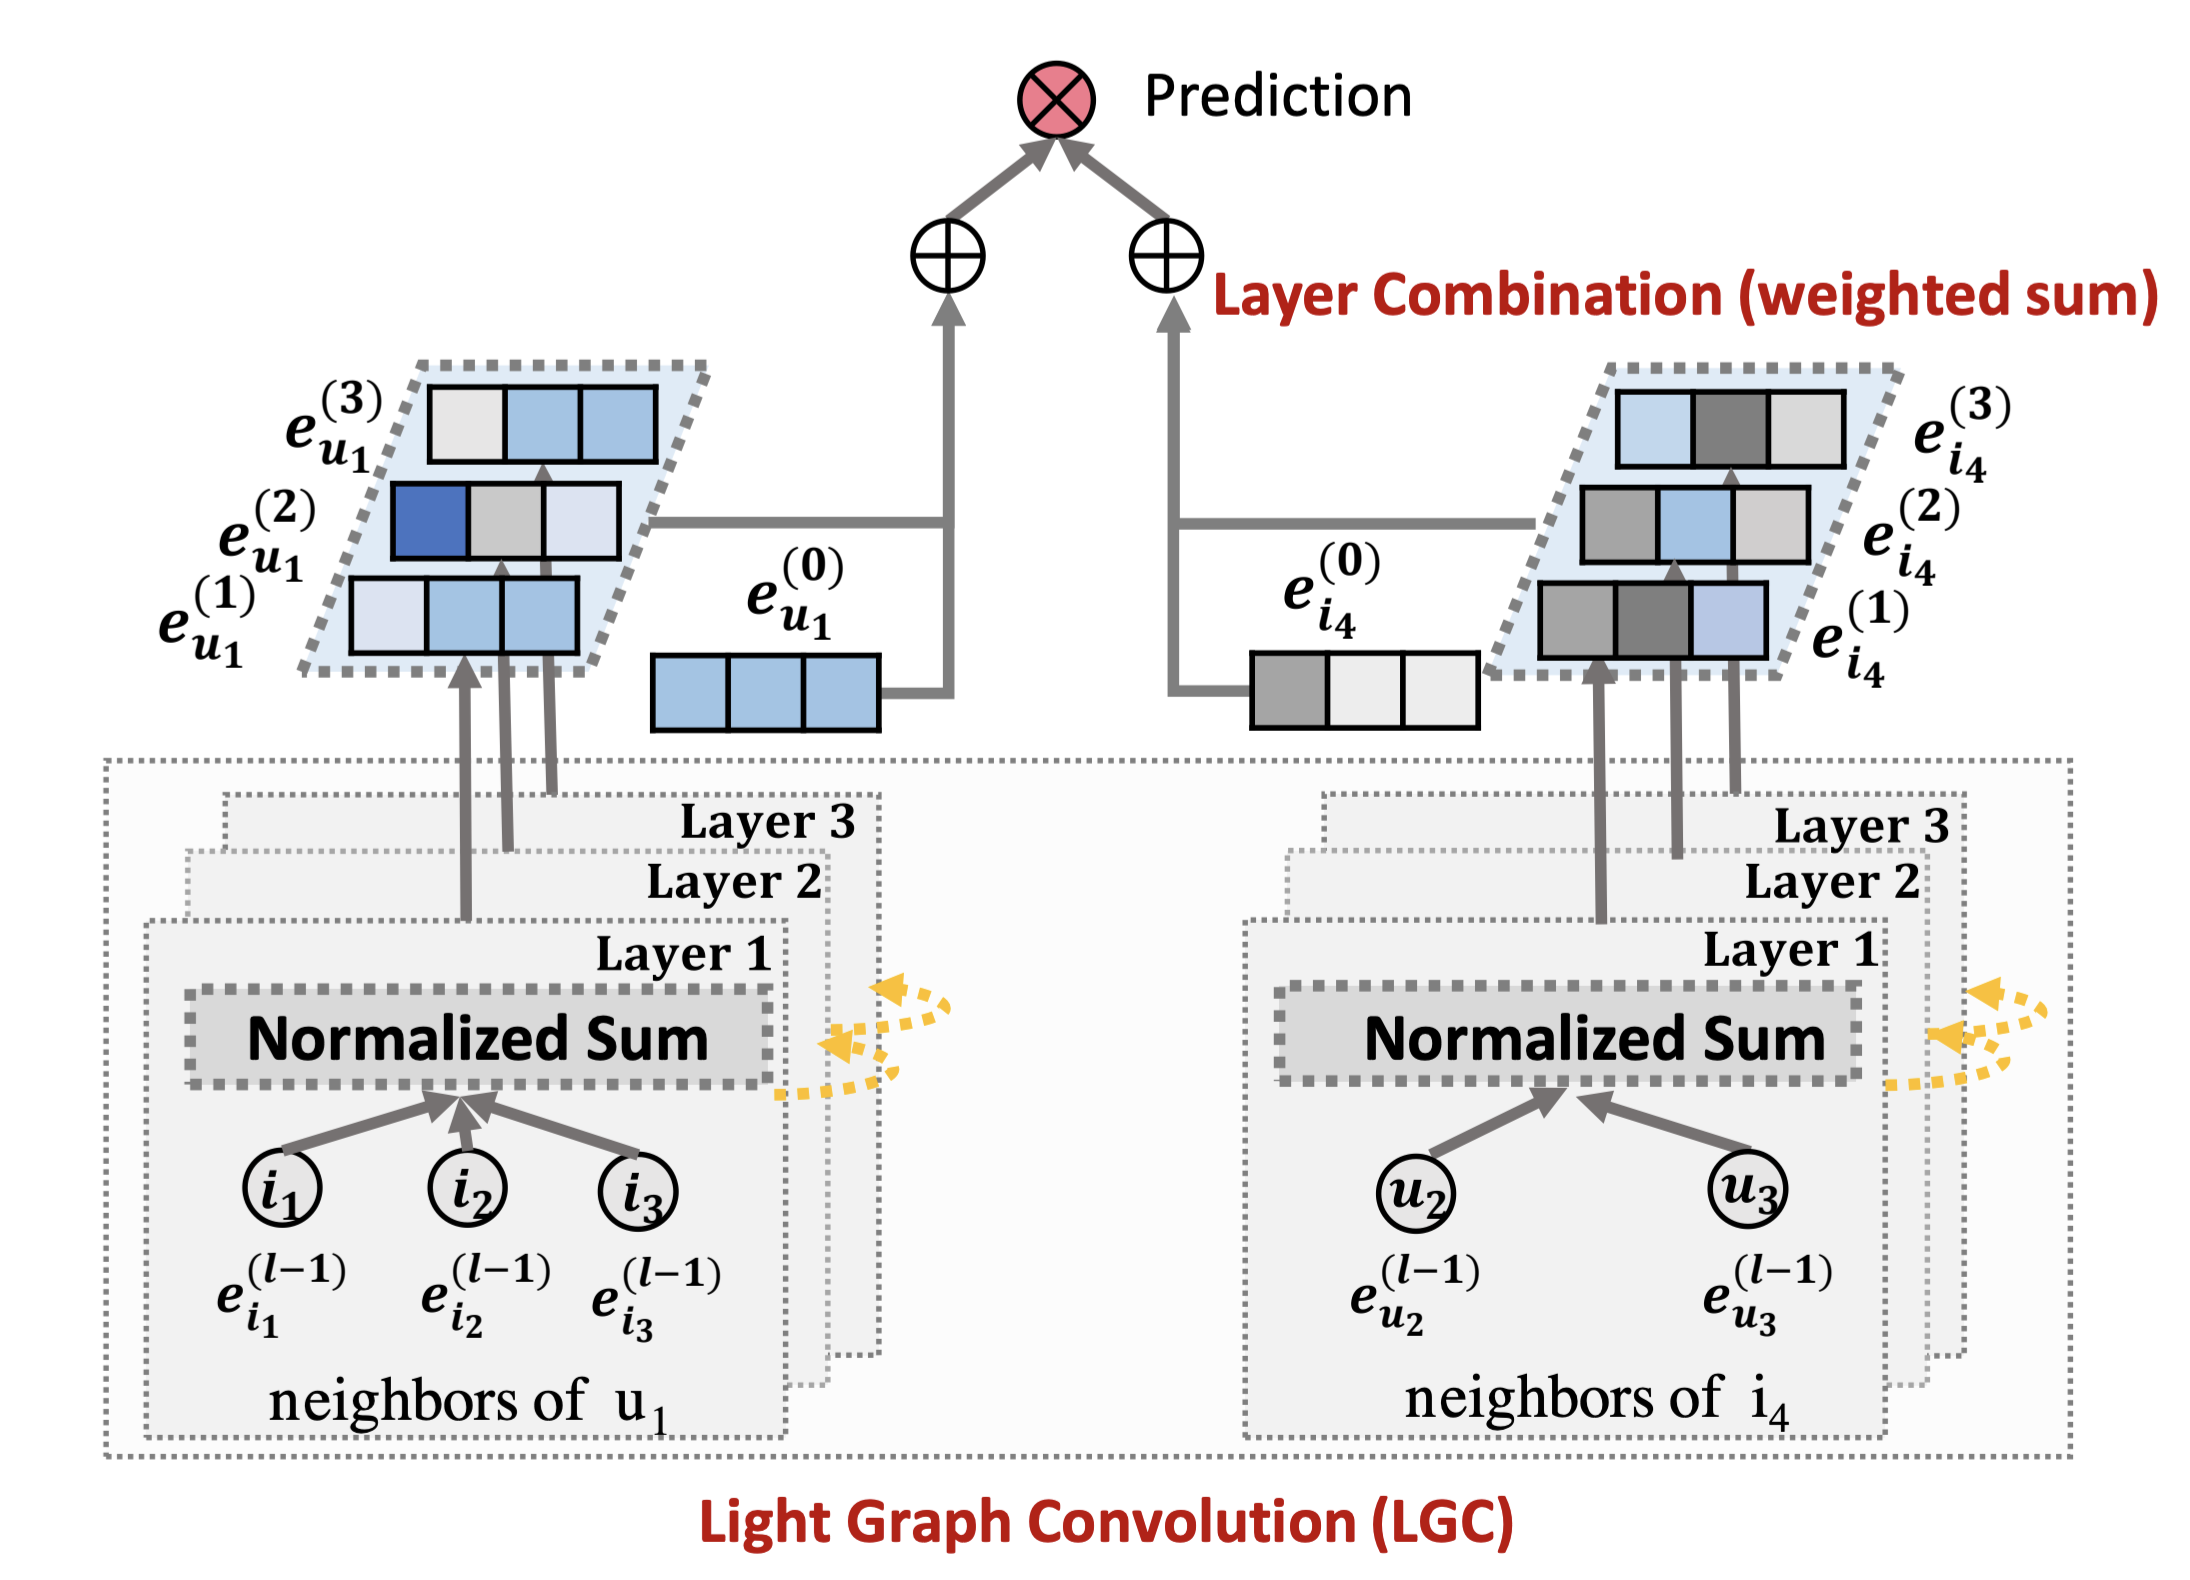
\includegraphics[width=\linewidth]{material/4.png}
    \caption{LightGCN Structure}
    \label{fig:4}
\end{figure}

\subsubsection{Training Process\newline}
Iterative optimization of the user and item embeddings is a part of the training procedure. Only positive user-item interactions are used to train the model; pairings with ratings of less than one are ignored. An embedding regularization term and a matrix factorization loss are combined in the training objective:

\[L = L_{MF} + \lambda L_{reg}\]

Where $L_MF$ is the matrix factorization loss based on the inner product of the embeddings of the user and item, and $L_reg$ is the L2 regularization term in the embeddings.

\subsubsection{Embeddings\newline}
LightGCN uses message passing on the user-item interaction network to create low-dimensional embeddings for both users and items (news articles). These embeddings function as concise representations for tasks downstream and capture intricate patterns of interaction. A weighted total of the embeddings from every layer is used to calculate the final embeddings:
\[e_{final} = \sum(\alpha_k * e_k)\]
Here $\alpha_k$ are the learnable weights for each layer's contribution.


\subsection{Method 5: Deep Learning Model}
This news recommendation system, which is based on deep learning, combines several feature representations and uses the neural network architecture to identify intricate patterns in user-news interactions. A detailed representation of the news material is produced by combining TF-IDF, entity embeddings, and category characteristics; the neural network then facilitates the learning of complex correlations between these aspects and user preferences.

\subsubsection{Model Type\newline}
LightGCN, a Graph Convolutional Network (GCN) streamlined for recommendation systems, is used in this model. Using the graph structure of user-item interactions, LightGCN explicitly incorporates both low-order and high-order connectivity patterns to learn the user and item embeddings.

\subsubsection{Data Input\newline}
A wide range of information from news items and user behaviour are ingested by the model. Text representation utilizing entity embeddings and TF-IDF vectorization, which allows for a maximum of 5000 features, combine to create these features. While entity embeddings are obtained using pretrained vectors associated with entities mentioned in the news stories, the text representation includes both news headlines and abstracts. Furthermore, one-hot encoding is used to encode categorical features such as news category and subcategory, which are then concatenated with the other data.

\subsubsection{Training Process\newline}
An Adam algorithm-optimized binary cross-entropy loss function is used to train the model. Iterating batches of news stories and the features that accompany them is part of the training process. While the sample code snippet supplied uses fictitious labels, in a real-world application, the labels would be generated by user-interaction data, indicating whether or not a user interacted with a certain news story.

\subsubsection{Embeddings\newline}
Pre-trained entity and relation embeddings are loaded from external files and utilised by the system. These embeddings capture semantic links and offer a dense vector representation of items referenced in news stories. The entity embeddings of every news article are combined by averaging all of the entity vectors connected to it, resulting in a fixed-length representation that is independent of the number of entities.

\subsubsection{Prediction Task\newline}
Predicting whether a user would interact with a certain news piece is the main goal of this model. The job is structured as a binary classification in which the model generates a score that represents the likelihood of user participation. During the suggestion process, cosine similarity is used to calculate how similar a user's profile, which is derived from their past interactions, is to potential news items. The user is then suggested to choose the top N articles with the highest similarity ratings.

\section{Evaluation}
The GNN and LibFM models could not be trained effectively due to training problems. As a result, the major topics of discussion in this part will be the training procedures and outcomes of the remaining three models.


\subsection{Neural Collaborative Filtering}
Figures \ref{fig:5} depict the evolution of two crucial performance measures during the model training process: the training loss and the validation AUC (Area Under the Curve). These measures offer vital information on the learning processes of the model and its ability to generalize to unfamiliar data. The training loss curve illustrates the model's performance on the training dataset throughout consecutive epochs, while the validation AUC curve measures the model's prediction accuracy on a distinct validation set, providing an indication of its capacity to generalize.

\begin{enumerate}
\item \textbf{Training Loss\newline}

The training loss shows a consistent downward trend, decreasing from an initial value of approximately 0.17 to about 0.03 by the 9th epoch.
The loss curve is relatively smooth with no significant fluctuations, indicating a stable learning process.
The continuous decrease in the loss value suggests that the model performance on the training set is steadily improving, demonstrating effective learning.


\item \textbf{Validation AUC (Area Under the Curve)\newline}

The validation AUC exhibits an overall upward trend, rising from an initial value of about 0.5 to approximately 0.95 by the ninth epoch.
The AUC curve remains relatively flat for the first few epochs, then shows a significant increase starting from the fourth epoch.
There is a notable jump between the sixth and seventh epochs, followed by continued steady improvement.


\item \textbf{Model Performance Analysis\newline}

The trends in training loss and validation AUC correspond well, indicating that the model is not only improving on the training set but also demonstrating good generalizability on the validation set.
The AUC value increasing from 0.5 (equivalent to random guessing) to nearly 0.95 suggests that the model has made significant progress in distinguishing between positive and negative samples.
There are no apparent signs of overfitting, as the validation AUC continues to rise without showing any downward trend.


\item \textbf{Training Process Characteristics\newline}

The model learning appears to be relatively slow in the first few epochs, possibly establishing initial feature representations.
The middle phase (epochs 4-7) shows accelerated learning, suggesting that the model may have found more effective feature combinations or optimization directions.
The later phase (epochs 7-9) shows slightly slower but continued improvement, possibly approaching an optimal solution.


\end{enumerate}

\begin{figure}
    \centering
    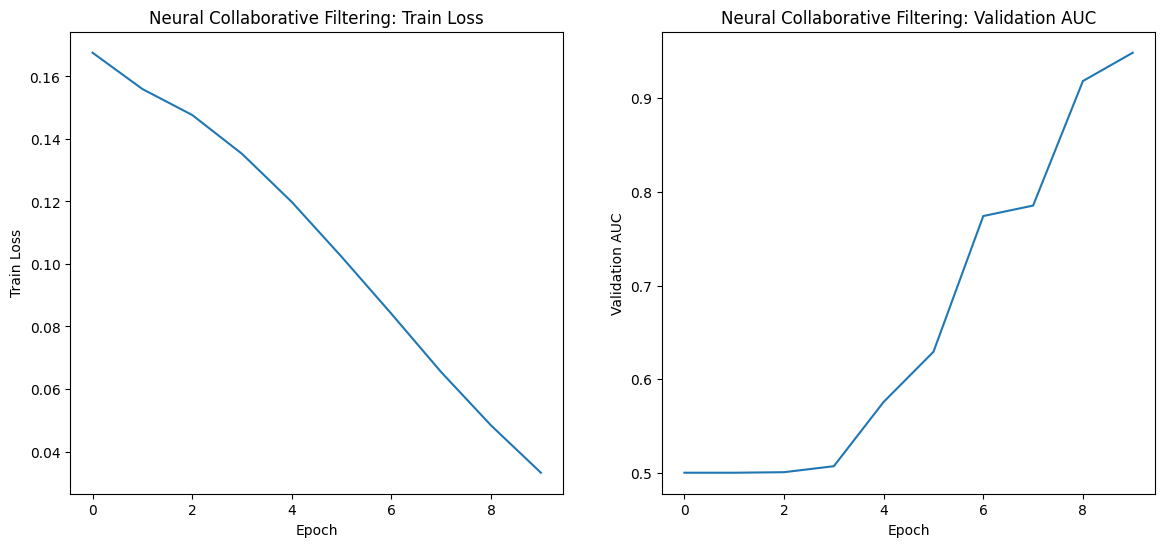
\includegraphics[width=\linewidth]{material/5.png}
    \caption{Neural Collaborative Filtering Training}
    \label{fig:5}
\end{figure}

In conclusion, the training process of this NCF model shows excellent performance, showcasing strong learning capabilities and generalization performance. It has successfully extracted effective collaborative filtering patterns from the data.

\subsection{Matrix factorization}
\begin{figure}
    \centering
    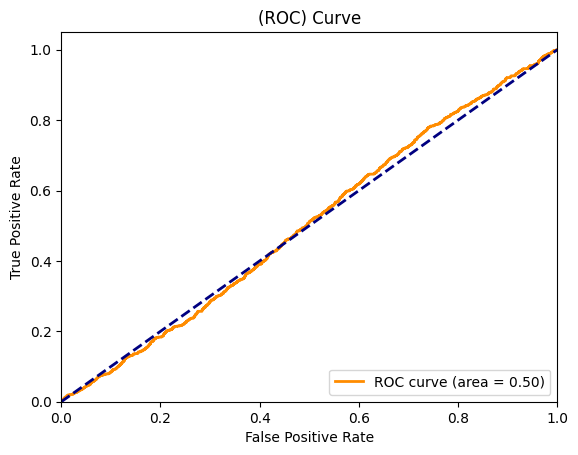
\includegraphics[width=\linewidth]{material/7.png}
    \caption{Deep Learning Model Training}
    \label{fig:6}
\end{figure}
This Figure \ref{fig:6} displays a Receiver Operating Characteristic (ROC) curve for Matrix factorization. The Receiver Operating Characteristic (ROC) curve is a crucial tool for assessing the effectiveness of models that classify data into two categories. The primary objectives of this are the following.

\begin{enumerate}
    \item The model classification performance is presented by the curve, which illustrates the relationship between the True Positive Rate and False Positive Rate at different classification levels.
    \item Evaluating the efficacy of different models: The quantification of the overall performance of the model may be achieved by computing the Area Under the Curve (AUC). A higher AUC value suggests superior model performance.
    \item Determining the most favourable threshold: The receiver operating characteristic (ROC) curve can assist in selecting the optimal classification threshold to achieve a balance between true positives and false positives.
    \item Evaluating the model's capacity to distinguish between different classes: The curvature of the curve indicates the model's capacity to differentiate between positive and negative samples.
\end{enumerate}

The graph displays the ROC curve as the solid orange line, while the dashed blue line shows the diagonal, which serves as the baseline for random guessing. The caption indicates that the area under the curve (AUC) is 0.50, suggesting that this model's performance is comparable to random guessing and lacks the ability to make accurate predictions. Optimally, we need a ROC curve that exhibits a substantial improvement over the diagonal line, with an AUC value approaching 1.

\subsection{Deep Learning Model}
\begin{figure}
    \centering
    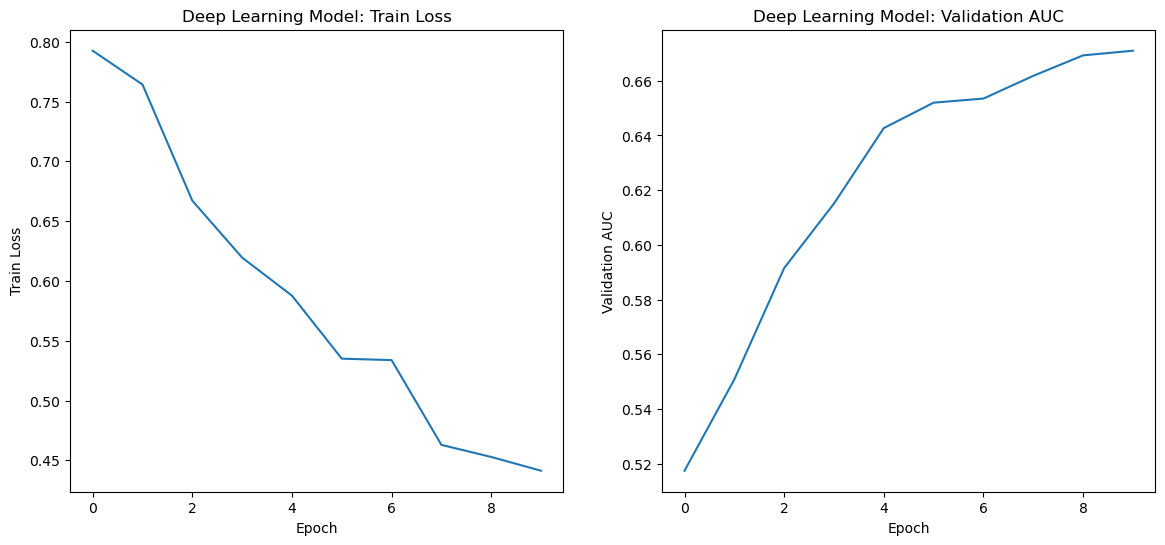
\includegraphics[width=\linewidth]{material/6.png}
    \caption{MF's Receiver Operating Characteristic curve}
    \label{fig:7}
\end{figure}
Figures \ref{fig:7} depict the evolution of two crucial performance measures during the model training process: the training loss and the validation AUC (Area Under the Curve).
\begin{enumerate}
    \item \textbf{Training Loss}
    \begin{itemize}
        \item Exhibits a persistent and continuous decline, commencing at around 0.80 and concluding at 0.45.
        \item The most pronounced fall takes place during the initial 3 epochs, followed by a more steady decline.
        \item A short period of stability may be observed between epochs 6 and 7.
    \end{itemize}
    \item \textbf{Validation AUC}
    \begin{itemize}
        \item Shows a consistent and gradual increase, starting at roughly 0.52 and reaching a value of approximately 0.67 by the conclusion of the observed period.
    
        \item There was a significant initial improvement in the first 4 epochs, which was then followed by slower progress.
        \item An inconspicuous decline can be observed in epochs 6-7, aligning with the period of stability in training loss.
    \end{itemize}
    The model has characteristic learning behavior, characterized by a rapid initial enhancement followed by gradual and incremental progress. The final validation AUC of 0.67 suggests a reasonable level of predictive performance, suggesting that there is potential for additional optimization. The persistent decrease in training loss, along with the diminishing enhancement in validation AUC, suggests the possibility of overfitting in the latter epochs.
\end{enumerate}

\subsection{Analyse}
The Table \ref{tab:4} show the result of the model on testing set.
\begin{enumerate}
    
\item \textbf{Matrix Factorisation (MF)\newline}
The Matrix Factorization model shows an AUC of 0.69, which indicates a moderate to good performance. However, the lack of other metrics makes it challenging to provide a comprehensive evaluation of this model's capabilities.
\item \textbf{Neural Collaborative Filtering (NCF)\newline}
The Neural Collaborative Filtering model demonstrates excellent performance with an AUC of 0.82. This is the highest AUC among the three models, suggesting superior predictive power. Unfortunately, the absence of other metrics prevents a more in-depth comparison with the other models.
\item \textbf{Deep Learing Models\newline}
The Deep Learning model presents an AUC of 0.62, indicating average performance. Its MRR of 0.34 is acceptable considering the relatively low AUC. The nDCG@5 of 0.42 and nDCG@10 of 0.61 suggest that the relevance of recommendations improves as the number of recommended items increases.
\end{enumerate}

AUC Comparison: NCF > MF > Deep learning

The NCF model clearly outperforms the others in distinguishing between relevant and irrelevant items.

Deep Learning Model Analysis:

Despite its lower AUC, the Deep Learning model achieves an nDCG\@10 of 0.61, indicating good relevance among the top 10 recommendations. The MRR of 0.34 suggests that, on average, the first relevant item appears around the third position (1/0.34 ≈ 2.94).

\section{Discussion}
\subsection{Factorisation Machines}

\begin{itemize}
    \item \textbf{High-Dimensional Sparse Data\newline}
    LibFM works very well with high-dimensional sparse datasets, which makes it a great fit for scenarios involving news recommendation where user-item interaction data is frequently sparse. Even with a few data points, learning may be accomplished effectively thanks to the model's efficient handling of sparsity.
    \item \textbf{Feature Interaction\newline}LibFM's ability to capture feature interactions is one of its main advantages over linear models in terms of expressiveness. This skill is essential for news recommendation, as an article's relevance to a user is frequently determined by intricate interactions between a number of characteristics, including topic, writing style, and user preferences.
\end{itemize}



\subsection{Neural Collaborative Filtering}

\begin{itemize}
    \item \textbf{Perceiving High-Dimensional Sparse Data\newline}News recommendation datasets typically contain high-dimensional sparse data, which NCF has an impressive capacity to perceive. Even with few user-item interactions, the model can extract significant patterns due to the neural network architecture's ability to interpret sparse input information effectively.
    \item \textbf{Embeddings for Interactions\newline}NCF can represent people and news items in a dense, low-dimensional space by using embeddings to capture interactions and extract information. This strategy makes it easier to find minute parallels and connections that conventional collaborative filtering techniques could miss.
    
    \item \textbf{Deep Learning Approach\newline}By integrating deep learning methods into NCF, the cooperative filtering procedure is improved. The model can develop hierarchical representations of persons and objects thanks to many layers of neural networks, which may help it capture more intricate and non-linear correlations in the data.
\end{itemize}

\subsection{Matrix factorization}

\begin{itemize}
    \item \textbf{Handling Sparse and Incomplete Data\newline}MF's success in handling sparse and incomplete datasets is noteworthy. Sparse and incomplete datasets are frequently encountered in news recommendation scenarios, when consumers engage with a small portion of the available articles. MF is able to deduce possible interactions even for objects that users have not explicitly evaluated by breaking down the user-item interaction matrix into lower-dimensional latent component matrices.
    \item \textbf{Dimensionality Reduction\newline}The complexity and dimensionality of the data are naturally decreased throughout the matrix factorisation process. This reduction helps find the most important aspects that influence user preferences and item qualities in addition to improving the computational process' efficiency.
    
    \item \textbf{Modeling Latent Factors\newline}When it comes to modelling latent variables in user-item interactions, MF is quite effective. These hidden variables might be abstract ideas that affect user preferences and item qualities but are not immediately apparent. This capacity enables a more in-depth comprehension of the fundamental trends in news consumption.

    \item \textbf{Overfitting and Underfitting\newline}Despite its advantages, MF can lead to overfitting and underfitting, particularly when the model's complexity exceeds the amount of data that is available. On the other hand, if the model is too basic to accurately represent the subtleties of user-item interactions, underfitting may result. In order to achieve optimal performance in news recommendation tasks, it is imperative to balance these characteristics through appropriate model selection and regularisation.
\end{itemize}

\subsection{Graph Neural Networks}
\begin{itemize}
    \item \textbf{Capturing Complex High-Order Relationships\newline} GNNs are particularly good at modelling complicated high-order interactions that exist between users and news items. GNNs are able to capture complex patterns of impact and similarity that extend beyond paired interactions by visualizing the recommendation issue as a graph, in which users and articles are nodes and interactions are edges.
    \item \textbf{Deeper Interactions\newline} Deeper interactions within the user-item graph may be modeled thanks to the message passing methods used by GNN. Using this method, information can spread across the network, perhaps revealing hidden relationships and enhancing the quality of suggestions, particularly for people or things with few direct interactions.
\end{itemize}

\subsection{Deep Learning Model}
\begin{itemize}
    \item \textbf{Manual Feature Design and Extraction\newline} The feature design and extraction process for this approach requires a significant amount of manual labour. Although this allows for adding domain-specific information, it can be laborious and may not be suitable for large, diversified news databases. The manual nature of this process also adds a degree of subjectivity, which could skew the recommendation algorithm.
    \item \textbf{Complicated Connections\newline} Entity embedding and TF-IDF alone might not be able to capture the intricate, non-linear interactions that exist between readers and news items. This constraint results from the pre-trained entity embeddings' static nature and TF-IDF's intrinsic linearity. Consequently, it is possible that minor variations in user preferences or content attributes go unnoticed, which could result in fewer customized suggestions.
\end{itemize}

\section{Future Work}
\begin{enumerate}
    \item \textbf{Optimised Feature Development\newline} In order to save human labour and enhance the capacity to extract and design features automatically, future studies should investigate automated techniques for feature extraction and design. This can involve utilizing cutting-edge machine learning methods, including automated feature selection algorithms or deep learning-based feature extraction, to find and produce pertinent characteristics more quickly and accurately.
    \item \textbf{Models Hybrids\newline} Future research should focus on creating hybrid approaches that integrate matrix factorisation with other methods. These hybrid models may be able to reduce the problems of both overfitting and underfitting while also increasing prediction accuracy. For example, combining matrix factorisation with ensemble techniques or deep learning architectures may result in recommendation systems that are more reliable and accurate.
    \item \textbf{Integrating Contextual Data\newline} To improve model performance, future research should concentrate on adding more contextual data, such as temporal dynamics, item features, and user demographics. Researchers may create more complex and individualized recommendation systems that take into consideration the complex interplay between user preferences and item features by using these rich data sources.
    \item \textbf{Improvements in Scalability\newline}Future developments in this area depend on looking at scalable algorithms and distributed computing strategies to manage large-scale datasets more effectively. To create algorithms that can process and analyze large volumes of data in real time or almost real time, researchers should investigate parallel processing frameworks such as distributed TensorFlow or Apache Spark.
    \item \textbf{Advanced Neural Network Techniques \Newline} Future study should focus on applying sophisticated neural network approaches, such as dynamic and hierarchical graph neural networks. More accurate and flexible recommendation systems may result from the use of these advanced models, which are better able to represent the intricate and dynamic relationships found in the data. In order to capitalize on their abilities to represent intricate connections, future research should investigate the integration of these cutting-edge neural network designs with already used recommendation systems.
\end{enumerate}

\section{Conclusion}
Based on the MIND (Microsoft News Dataset) dataset, this research project has successfully built and evaluated a comprehensive news recommendation engine. We have performed a thorough review of their effectiveness in recommending news items to consumers based on their past interactions and preferences using a wide range of approaches. The multimodal methodology in this study has produced insightful information about the intricacies of news recommendation algorithms and how they could improve user engagement on digital news platforms.

We have made a substantial contribution to the field of personalised news recommendation by methodically exploring each strategy and identifying and clarifying its strengths and limits. The range of approaches examined, from more complex methods like Graph Neural Networks (GNNs) to more conventional approaches like entity embedding and Term Frequency-Inverse Document Frequency (TF-IDF), highlights the intricate nature and subtle considerations needed in creating successful recommendation systems. We have been able to thoroughly evaluate the trade-offs between computational complexity, prediction accuracy, and scalability across many recommendation paradigms because to this varied methodological environment.

Our results indicate that although each approach shows distinct benefits in particular scenarios, there is still a significant amount of room for development in the recommendation system in a number of areas. Advanced feature engineering techniques, hybrid models that incorporate various approaches in a synergistic way, and improving scalability to support large-scale, real-time news recommendation situations are particularly attractive topics for future study and development. These prospective upgrades might greatly increase the system's ability to provide extremely precise and personalized suggestions, which would increase user engagement and happiness with digital news platforms.

Furthermore, this work has brought to light the importance of striking a balance between algorithmic complexity and practical implementability in real-world news recommendation scenarios. Our comparison investigation yielded valuable insights that will serve as a strong basis foxr further research endeavours focused on improving and streamlining news recommendation systems. The creation of more flexible, effective, and user-focused recommendation algorithms will be crucial in determining how people interact and consume news in the digital era as the landscape of digital news continues to change.
% sdd

\begin{table*}[p]
\centering
\caption{Number of samples in dataset}
\begin{tableminipage}{\textwidth}
\begin{tabularx}{\textwidth}{@{}XXXX@{}}
\hline
{\bf Dataset} & {\bf \texttt{behaviors.tsv}} & {\bf \texttt{news.tsv}} \\
\hline
Training set &	2,232,748  &	711,222\\
Validation set &	376,471  &	72,023\\
Test set &	2,370,727  &	120,959\\
\hline
\end{tabularx}
  \label{tab:1}
\end{tableminipage}
\end{table*}


\begin{table*}[p]
\centering
\caption{First 5 rows of the \texttt{behaviors.tsv} file in the training set}
\begin{tableminipage}{\textwidth}
\begin{tabularx}{\textwidth}{@{}cXXXXXX@{}}
\hline
{} & {\bf Impression\_ID} & {\bf User\_ID} & {\bf Time} & {\bf History} & {\bf Impressions} \\
\hline
0 & 1 & U87243 & 11/10/2019 11:30:54 AM & N8668 N39081 N65259 N79529 N73408 N43615 N2937... & N78206-0 N26368-0 N7578-0 N58592-0 N19858-0 N5...\\
1 & 2 & U598644 & 11/12/2019 1:45:29 PM & N56056 N8726 N70353 N67998 N83823 N111108 N107... & N47996-0 N82719-0 N117066-0 N8491-0 N123784-0 ...\\
2 & 3 & U532401 & 11/13/2019 11:23:03 AM & N128643 N87446 N122948 N9375 N82348 N129412 N5... & N103852-0 N53474-0 N127836-0 N47925-1\\
3 & 4 & U593596 & 11/12/2019 12:24:09 PM & N31043 N39592 N4104 N8223 N114581 N92747 N1207... & N38902-0 N76434-0 N71593-0 N100073-0 N108736-0...\\
4 & 5 & U239687 & 11/14/2019 8:03:01 PM & N65250 N122359 N71723 N53796 N41663 N41484 N11... & N76209-0 N48841-0 N67937-0 N62235-0 N6307-0 N3...\\
\hline
\end{tabularx}
  \label{tab:2}
\end{tableminipage}
\end{table*}

\begin{table*}[p]
\centering
\caption{First 5 rows of the \texttt{news.tsv} file in the training set}
\begin{tableminipage}{\textwidth}
\begin{tabularx}{\textwidth}{@{}cXXXXXXXX@{}}
\hline
{} & {\bf News\_ID} & {\bf Category} & {\bf Subcategory} & {\bf Title} & {\bf Abstract} & {\bf URL} & {\bf Title\_Entities} & {\bf Abstract\_Entities}\\
\hline
0 & N88753 & lifestyle & lifestyleroyals & The Brands Queen Elizabeth, Prince Charles, an... & Shop the notebooks, jackets, and more that the... & https://assets .msn.com/ labs/mind /AAGH0ET .html & \texttt{[\{"Label": "Prince Philip, Duke of Edinburgh",...]} & \texttt{[]}\\
1 & N45436 & news & newsscience-andtechnology & Walmart Slashes Prices on Last-Generation iPads & Apple's new iPad releases bring big deals on l... & https://assets .msn.com/ labs/mind/ AABmf2I.html & \texttt{[\{"Label": "IPad", "Type": "J", "WikidataId": ...]} & \texttt{[\{"Label": "IPad", "Type": "J", "WikidataId": ...}\\
2 & N23144 & health & weightloss & 50 Worst Habits For Belly Fat & These seemingly harmless habits are holding yo... & https://assets .msn.com/ labs/mind/ AAB19MK.html & \texttt{[\{"Label": "Adipose tissue", "Type": "C", "Wik...]} & \texttt{[\{"Label": "Adipose tissue", "Type": "C", "Wik...]}\\
3 & N86255 & health & medical & Dispose of unwanted prescription drugs during ... & NaN & https://assets .msn.com/ labs/mind/ AAISxPN.html & \texttt{[\{"Label": "Drug Enforcement Administration", ...]} & \texttt{[]}\\
4 & N93187 & news & newsworld & The Cost of Trump's Aid Freeze in the Trenches... & Lt. Ivan Molchanets peeked over a parapet of s... & https://assets .msn.com/ labs/mind/ AAJgNsz.html & \texttt{[]} & \texttt{[\{"Label": "Ukraine", "Type": "G", "WikidataId...]}\\
\hline
\end{tabularx}
  \label{tab:3}
\end{tableminipage}
\end{table*}

\begin{table*}[p]
\centering
\caption{Result}
\begin{tableminipage}{\textwidth}
\begin{tabularx}{\textwidth}{@{}XXXXX@{}}
\hline
{\bf Model} & {\bf AUC} & {\bf MRR} & {\bf nDCG@5} & {\bf nDCG@10} \\
\hline
MF & 0.69  &	 &  &\\
NCF & 0.82  &	&  & \\
Deep Learing &	0.62  &	0.34 & 0.42 & 0.61\\
\hline
\end{tabularx}
  \label{tab:4}
\end{tableminipage}
\end{table*}

\nocite{*}
\bibliography{References}


\end{document} 